\section{System Design}

To address the three failures identified in Section~1, we design CLIO Search around two central principles: science-aware operators must execute as first-class retrieval branches, and an agentic orchestration layer must reason about \emph{what} to search before executing. The architecture comprises a staged pipeline with four parallel branches (Sec.~3.1), dimensional conversion operators that perform explicit SI arithmetic (Sec.~3.2), deterministic formula normalization (Sec.~3.3), a hybrid fusion strategy (Sec.~3.4), federated multi-namespace search (Sec.~3.5), and an agentic orchestration layer with corpus profiling, adaptive branch selection, and multi-hop refinement (Sec.~3.6).

\subsection{Architecture Overview}

\begin{figure}[!t]
\centering
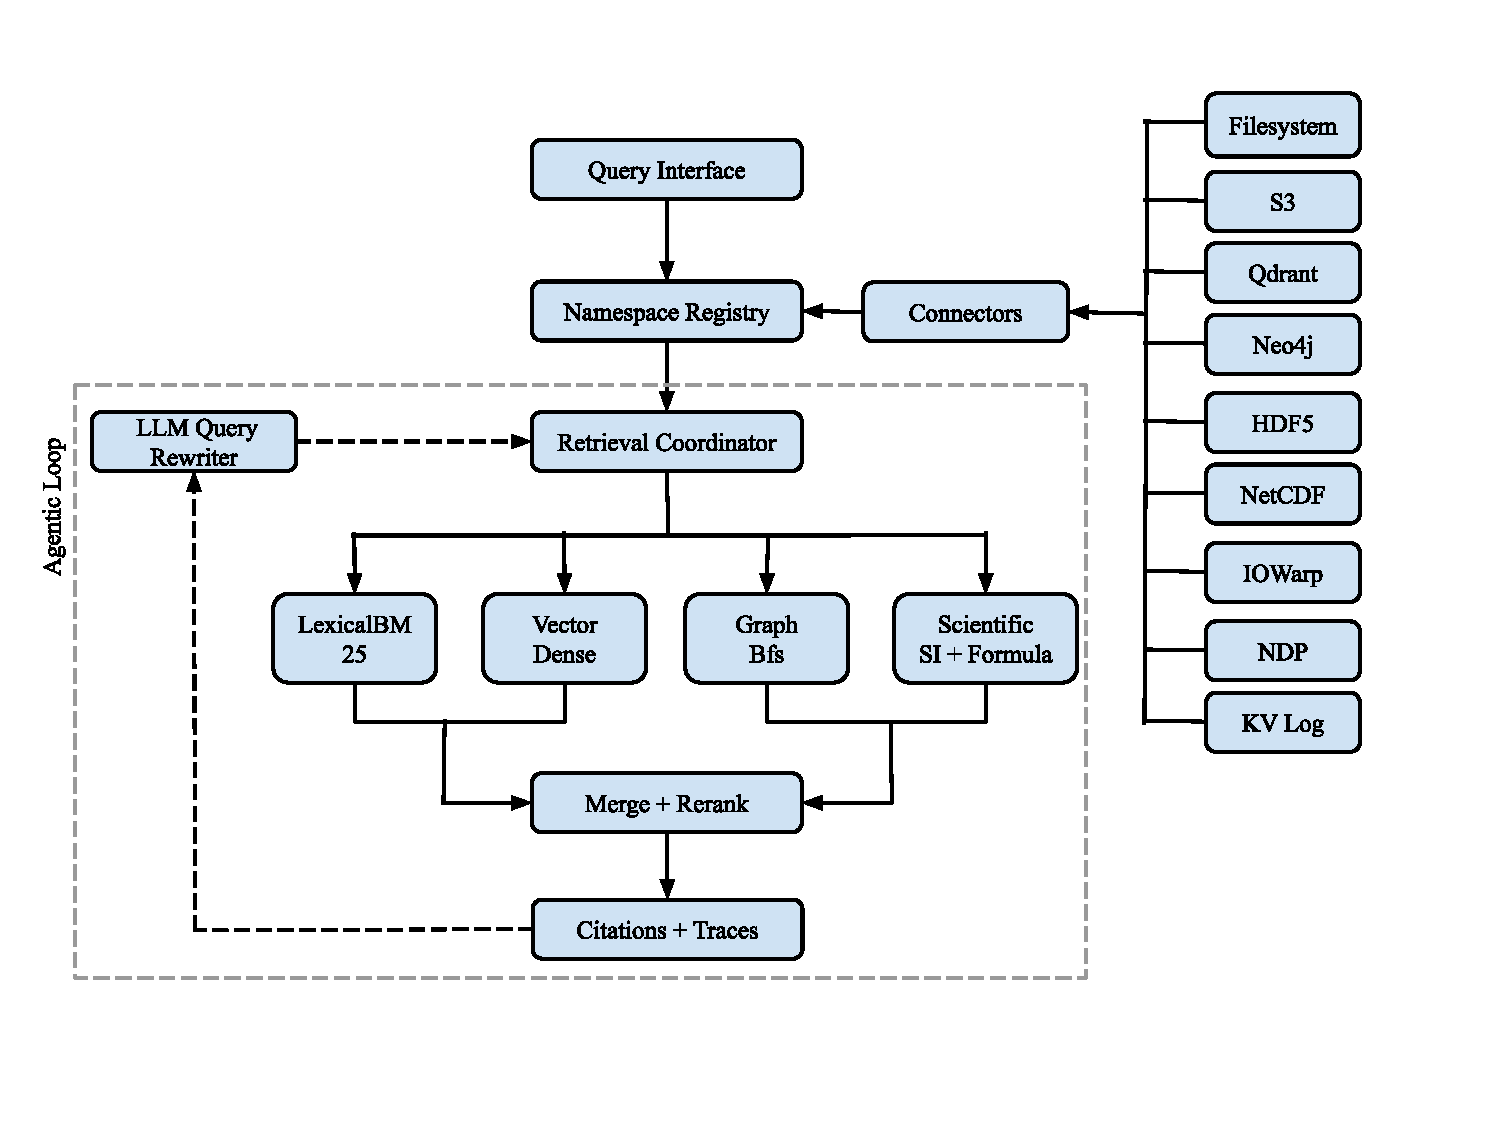
\includegraphics[width=\columnwidth]{figures/architecture.pdf}
\caption{System architecture of \textsc{clio-agentic-search}. Nine connectors
mediate heterogeneous backends; science-aware components execute alongside
standard retrieval branches. The agentic loop iteratively refines queries
via LLM rewriting.}
\label{fig:architecture}
\end{figure}

The system is a staged pipeline with four parallel retrieval branches (Fig.~\ref{fig:architecture}). A query enters through the Query Interface (FastAPI REST endpoint or CLI), which parses the raw query string, extracts typed scientific constraints (numeric ranges, unit filters, formula patterns), and forwards a structured query object to the Namespace Registry. The registry resolves which namespaces---each backed by one of six connector types---are eligible for the query based on capability negotiation (Sec.~3.5).

The Retrieval Coordinator fans the query out to four parallel branches: lexical (BM25), vector (dense embedding similarity), graph (entity-relationship traversal), and scientific (dimensional measurement and formula queries). Each branch executes independently and returns scored candidate chunks. The Merge and Rerank stage deduplicates candidates by chunk identifier, applies hard scientific filters, computes a composite score via heuristic fusion, and emits the final top-$K$ results with source citations.

Nine connectors mediate access to heterogeneous backends: local filesystem, S3-compatible object stores, Qdrant vector database, Neo4j graph database, HDF5 (via h5py), NetCDF (via xarray), IOWarp CTE blob storage, NDP catalog (via MCP), and a key-value log store. Each connector declares a capability set specifying which retrieval branches it supports, enabling the coordinator to skip unsupported branches rather than fail. The IOWarp connector indexes scientific metadata from CTE blobs at ingest time and answers cross-unit queries against the DuckDB index; the NDP connector discovers and indexes datasets from the National Data Platform via the Model Context Protocol. Every pipeline stage emits structured trace events for observability.

\subsection{Dimensional Conversion Operators}

The core insight behind dimensional conversion is that cross-unit matching is an arithmetic problem, not a similarity problem. When a scientist queries for pressures between 190 and 360 kPa, the system must recognize that a document reporting ``250000 Pa'' falls within that range. This requires multiplying 190 by 1000 to obtain 190000 Pa and 360 by 1000 to obtain 360000 Pa---a computation that no string normalization or learned embedding can guarantee.

The key insight underlying our approach is that physical units are not a flat enumeration---they are expressions over a small set of base dimensions. Every unit is fully characterized by a \emph{dimension vector} over the seven SI base dimensions $[\text{M}, \text{L}, \text{T}, \text{I}, \Theta, \text{N}, \text{J}]$ (mass, length, time, electric current, temperature, amount of substance, luminous intensity) plus a scale factor and optional offset relative to the SI base unit for that dimension combination. For example, Pa and kPa share the dimension vector $\text{M}^1\text{L}^{-1}\text{T}^{-2}$ with scale factors 1 and $10^3$ respectively. Two units are \emph{compatible} if and only if their dimension vectors are equal; \emph{conversion} between compatible units is the ratio of their scale factors.

We implement this as a composable unit registry (Table~\ref{tab:si_conversion}). Each entry is a 4-tuple: (dimension vector, scale, offset, domain tag). Adding a new unit requires adding a single configuration entry---no code changes. The domain tag disambiguates dimensionally identical but physically distinct quantities: becquerel (Bq) and hertz (Hz) are both $\text{T}^{-1}$, but a cross-unit radioactivity query should not match frequency measurements. At index time, a regex-based measurement extractor identifies numeric-unit pairs in document text and scientific file metadata. Each extracted measurement is stored as a 4-tuple: (raw\_value, raw\_unit, canonical\_value, dimension\_key). These tuples populate a \texttt{scientific\_measurements} table in DuckDB, indexed on canonical\_value and dimension\_key for efficient range scans.

\begin{table}[!t]
\centering
\caption{Composable unit registry: 46 units across 12 domains. Each unit is a dimension vector $[\text{M},\text{L},\text{T},\text{I},\Theta,\text{N},\text{J}]$ + scale factor. Adding a unit = adding one row.}
\label{tab:si_conversion}
\footnotesize
\renewcommand{\arraystretch}{1.15}
\setlength{\tabcolsep}{3pt}
\begin{tabular}{l l l c}
\toprule
\textbf{Domain} & \textbf{Dim.\ Vector} & \textbf{Units} & \textbf{Count} \\
\midrule
Length       & $\text{L}^1$                          & nm, mm, cm, m, km         & 5 \\
\rowcolor{gray!5}
Mass         & $\text{M}^1$                          & mg, g, kg                 & 3 \\
Time         & $\text{T}^1$                          & s, min, h                 & 3 \\
\rowcolor{gray!5}
Temperature  & $\Theta^1$                            & K, degC, degF             & 5 \\
Pressure     & $\text{M}^1\text{L}^{-1}\text{T}^{-2}$ & Pa, hPa, kPa, MPa, bar, atm, psi & 7 \\
\rowcolor{gray!5}
Velocity     & $\text{L}^1\text{T}^{-1}$            & m/s, km/h, kn             & 3 \\
Frequency    & $\text{T}^{-1}$                       & Hz, kHz, MHz, GHz, rad/s  & 5 \\
\rowcolor{gray!5}
Radioactivity & $\text{T}^{-1}$                      & Bq, Ci                    & 2 \\
Energy       & $\text{M}^1\text{L}^2\text{T}^{-2}$  & eV, keV, MeV, GeV, kJ, MJ, GJ & 7 \\
\rowcolor{gray!5}
Power        & $\text{M}^1\text{L}^2\text{T}^{-3}$  & W, kW, MW, GW             & 4 \\
Area         & $\text{L}^2$                          & ha                        & 1 \\
\rowcolor{gray!5}
Acceleration & $\text{L}^1\text{T}^{-2}$            & m/s$^2$                   & 1 \\
\midrule
\multicolumn{3}{l}{\textbf{Total}} & \textbf{46} \\
\bottomrule
\end{tabular}
\renewcommand{\arraystretch}{1.15}
\end{table}

At query time, three operators execute against the canonicalized measurement store. The \textbf{numeric-range} operator converts query bounds to the canonical scale for the query unit's dimension vector and issues a DuckDB range predicate: a query ``190:360:kPa'' becomes a scan for canonical\_value between 190000 and 360000 with dimension\_key = $\text{M}^1\text{L}^{-1}\text{T}^{-2}$. Because all pressure units---Pa, hPa, kPa, MPa, bar, atm, psi---share this dimension vector, a single index scan matches measurements originally expressed in \emph{any} pressure unit. The \textbf{unit-match} operator filters chunks containing any measurement with a compatible dimension vector. The \textbf{value-match} operator retrieves measurements matching a specific canonical value within a configurable tolerance (default $\pm$1\%).

The composability of this design merits emphasis. Becquerel (Bq) and curie (Ci) are both $\text{T}^{-1}$ with scale factors 1 and $3.7 \times 10^{10}$; adding curie is a single registry entry, and cross-unit radioactivity queries work automatically. Hertz is also $\text{T}^{-1}$, but the domain tag prevents radioactivity queries from matching frequency. The same principle extends to any unit expressible as a product of SI base dimensions---electromagnetic quantities, chemical concentrations, or domain-specific units---without code changes.

Correctness is guaranteed by construction: if the scale factor is correct, the match is correct. String normalization cannot bridge ``kilopascal'' and ``pascal''; learned embeddings~\cite{cone2026} achieve only 0.54 binary retrieval accuracy on numerical content~\cite{numeracygap2026}. Our guarantee depends on (1)~the extractor correctly identifying numeric-unit pairs and (2)~the registry covering the unit in question.

\subsection{Formula Normalization}

Scientific formulas appear in inconsistent surface forms across documents. ``$F = m \ast a$'', ``$F=ma$'', ``$F = m \cdot a$'', and ``$ma = F$'' express the same physical law but produce distinct token sequences that defeat both keyword and embedding retrieval. We normalize formulas through a deterministic six-step pipeline.

First, all whitespace is stripped. Second, all alphabetic characters are lowercased. Third, superscript notations are unified: LaTeX-style \texttt{\^{}\{N\}} and Python-style \texttt{**N} are both normalized to \texttt{\^{}N}. Fourth, the expression is split on the equality sign into left-hand and right-hand sides. Fifth, within each side, multiplicative factors are sorted lexicographically, so that \texttt{m*a} and \texttt{a*m} produce the same canonical form. Sixth, the two sides are rejoined with a normalized equality separator. The canonical form of all four variants above is \texttt{a*m=f}.

Normalized formulas are stored in a \texttt{scientific\_formulas} table in DuckDB alongside their source chunk identifiers and the raw original text. At query time, the user's formula expression passes through the same six-step pipeline before lookup. Formula matching integrates with the dimensional conversion operators as a parallel branch in the scientific retrieval stage: a query can simultaneously request formulas containing a specific equation and measurements within a numeric range, and both constraints execute as independent DuckDB queries whose results are intersected at the merge stage.

\subsection{Hybrid Retrieval Pipeline}

The retrieval pipeline executes four branches in parallel and merges their results through a deterministic fusion strategy.

\textbf{Lexical branch.} BM25 with parameters $k_1 = 1.2$ and $b = 0.75$ scores term overlap between query and document chunks, retrieving $\text{top\_k} \times 4$ candidates to provide recall headroom for downstream filtering.

\textbf{Vector branch.} Chunks are embedded with MiniLM-L6-v2 (384-dimensional vectors, cosine similarity) and indexed in Qdrant. This branch retrieves $\text{top\_k} \times 4$ candidates.

\textbf{Graph branch.} For Neo4j-backed namespaces, breadth-first traversal at depth 1 from query entities retrieves related chunks through typed relationships (e.g., cites, measures, uses\_formula). This branch retrieves $\text{top\_k} \times 2$ candidates, as graph neighborhoods are inherently more targeted.

\textbf{Scientific branch.} The dimensional conversion and formula normalization operators (Secs.~3.2--3.3) execute against DuckDB, returning $\text{top\_k} \times 4$ candidates from measurement range queries, unit-match filters, value-match lookups, and formula lookups.

\textbf{Merge and rerank.} Candidates from all branches are deduplicated by chunk\_id, retaining the maximum per-branch score. A scientific hard filter then applies: if the query specifies a numeric range or unit constraint, candidates not returned by the scientific branch are discarded---dimensional correctness is enforced, not merely preferred. A metadata filter removes candidates violating explicit metadata constraints (e.g., date range, file type). Surviving candidates are scored by a configurable weighted sum of branch scores (lexical, vector, metadata, scientific), with weights tunable per deployment. The top-$K$ candidates by composite score constitute the final result set. Each result carries provenance: the source namespace, chunk identifier, file path, and the set of branches that contributed to its retrieval.

\subsection{Federated Multi-Namespace Search}

Scientific data at HPC facilities spans heterogeneous backends. A single experimental campaign may deposit raw output on a parallel filesystem, preprocessed arrays in HDF5, derived features in a vector database, and annotations in a knowledge graph. Rather than require data migration, we bring the retrieval operators to the data.

Every storage backend is wrapped by a connector that implements the \texttt{NamespaceConnector} protocol and declares which retrieval capabilities it supports via runtime-checkable protocols (\texttt{LexicalSearchCapable}, \texttt{VectorSearchCapable}, \texttt{ScientificSearchCapable}, \texttt{GraphSearchCapable}, \texttt{CorpusProfileCapable}). The capability matrix is: Filesystem, S3, and IOWarp connectors support lexical, vector, scientific, and corpus profiling; NDP supports lexical and scientific; Qdrant supports vector search; Neo4j supports graph traversal; HDF5 and NetCDF support metadata and scientific search.

The Retrieval Coordinator consults this matrix before dispatching. When a query spans multiple namespaces, the coordinator executes the single-namespace pipeline independently for each namespace, activating only the branches that the namespace's connector supports. Results from all namespaces are collected into a global candidate pool, sorted by composite score, deduplicated by chunk\_id (since the same document may appear in multiple backends), and truncated to the final top-$K$.

Incremental indexing avoids redundant reprocessing. Each connector tracks indexed documents by SHA-256 content hash and modification time. On re-index, only documents whose hash or mtime has changed are reprocessed, enabling efficient index maintenance over evolving corpora without full rebuild.

\subsection{Agentic Orchestration}

Scientific data discovery at scale requires more than retrieval---it requires reasoning about \emph{what} to search, \emph{where} to search, and \emph{how} to search. Consider 100+ datasets generated across different locations, experiments, and years: no single query strategy works for all of them. Some data has rich metadata with explicit units; some has none. The agent must reason about how to access and interpret each dataset. We implement this through a four-stage agentic pipeline: \textbf{Discover}, \textbf{Reason}, \textbf{Transform \& Search}, and \textbf{Execute}.

\textbf{Stage 1: Discover (Corpus Profiling).} Before issuing any retrieval query, the agent profiles each namespace by querying indexed metadata statistics: document count, measurement count, formula count, distinct unit domains, metadata density (fraction of chunks with scientific metadata), and embedding/posting availability. This profiling executes as lightweight SQL aggregations against the existing DuckDB tables (no schema changes) and completes in under 12ms for a 210-document corpus. The profile answers: \emph{what is in this namespace, and what search strategies are viable?}

\textbf{Stage 2: Reason (Adaptive Strategy Selection).} The agent uses the corpus profile to make three decisions. First, \emph{branch selection}: if the corpus has no measurements, the scientific branch is skipped; if no embeddings are indexed, the vector branch is skipped. On our benchmark, this achieves 95.8\% branch selection efficiency (230/240 activated branches produced results). Second, \emph{metadata-adaptive strategy}: namespaces with metadata density above 50\% are tagged ``metadata-rich'' and queried with scientific operators; sparse namespaces fall back to lexical-heavy search. Third, \emph{namespace routing}: for multi-namespace queries, namespaces are scored by relevance (measurement availability, metadata density, formula coverage) and queried in priority order---the most relevant namespace first, with widening to additional namespaces in subsequent hops only if results are insufficient.

\textbf{Stage 3: Transform \& Search.} The science-aware operators (Secs.~3.2--3.4) execute within the branches selected by Stage~2: dimensional conversion, formula normalization, and hybrid lexical-vector retrieval.

\textbf{Stage 4: Execute (Multi-hop Refinement).} Retrieved results, along with the query and retrieval trace, are passed to an LLM (or deterministic fallback) that selects one of four strategies: \textbf{expand}, \textbf{narrow}, \textbf{pivot}, or \textbf{done}. If not done, the rewritten query re-enters the pipeline. Results from all hops are merged, deduplicated, and re-ranked. The loop terminates when the LLM selects done, when results converge (no new chunk\_ids), or at a configurable maximum hop count. Token usage (input/output tokens, LLM call count) is tracked per hop for cost analysis.

The critical architectural point is the separation between \emph{reasoning about what to search} and \emph{executing the search}. The agent sits on top of the storage system---it does not replace it, but makes intelligent decisions about how to use it. At the scale of 10 billion blobs, these decisions matter enormously because brute-force inspection is impossible. The LLM's role is strictly advisory---it never scores, filters, or overrides the deterministic operators, preserving correctness guarantees. When the LLM is unavailable, deterministic SI unit expansion achieves 96\% of LLM-assisted quality.

%% ===================================================================
%% Section 4: Implementation
